\begin{figure*}[t]
    \centering
    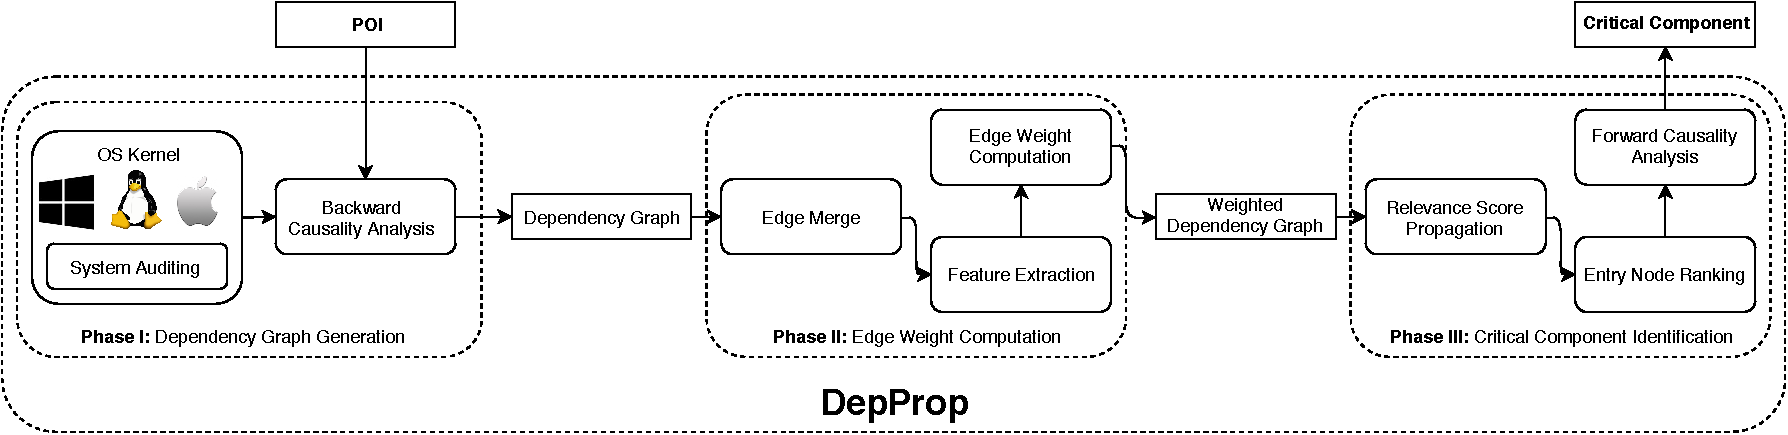
\includegraphics[width=0.95\textwidth,clip]{figs/architecture.pdf}
    \caption{The architecture of \tool}
    \label{fig:architecture}
\end{figure*}


\section{Overview}
\label{sec:overview}

%https://drive.google.com/file/d/1RE_n6d_rl2ciDsmN1IP0uVZJYl30NIG0/view?usp=sharing


\cref{fig:architecture} illustrates the architecture of \tool.
%
Given a POI, \tool employs techniques to automatically identify which parts of the backward dependency graph are actually relevant (referred to as ``critical component").
\tool consists of three phases: (1) dependency graph generation, (2) edge weight computation, and (3) critical component identification.
%
In Phase I, \tool leverages mature system auditing frameworks~\cite{auditd,etw,dtrace,sysdig}
%(\eg auditd~\cite{auditd}, ETW~\cite{etw}, DTrace~\cite{dtrace}, and Sysdig~\cite{sysdig}) 
to collect system-level audit logs about system calls (\cref{subsubsec:system-auditing}).
Given a POI event, \tool parses the collected logs and performs backward causality analysis~\cite{backtracking,backtracking2} to generate a backward dependency graph for POI (\cref{subsubsec:backward-causality}).

%
In Phase II, \tool first employs state-of-the-art dependency graph reduction techniques~\cite{reduction} to reduce the graph size
%by merging the same type of edges between two nodes that occur within a time window threshold 
(\cref{subsubsec:edge-merge}).
Then, \tool extracts features for edges (\cref{subsubsec:feature-extraction})
%that model the relevance of the edge to POI , 
and employs a \emph{discriminative feature projection scheme} to compute edge weights (\cref{subsubsec:weight-computation}), so that edges that are more relevant to POI (referred to as ``critical edges") can be better revealed. 
The output of Phase II is a weighted dependency graph for POI.

%
In Phase III, \tool first employs a \emph{relevance score propagation} scheme to propagate score backward from POI to entry nodes (\ie nodes without incoming edges) along the weighted edges (\cref{subsubsec:propagation}).
Then, \tool ranks entry nodes based on their POI relevance scores and selects the top-$k$ candidates (\cref{subsubsec:entry-ranking}).
Finally, \tool performs forward causality analysis from the selected entry node candidates, and identifies the overlap of the backward dependency graph and the forward dependency graph as the critical component for output (\cref{subsubsec:forward-causality}). 
Compared to the original backward dependency graph, the critical component contains the parts of dependencies that are actually relevant to POI and its size is significantly reduced, which facilitates further forensic investigation.


%\pgao{poi event <-> poi node}




\myparatight{Threat Model}
Our threat model follows the threat model of previous work on system monitoring~\cite{backtracking,backtracking2,loggc,trustkernel,gao2018aiql,gao2018saql,liu2018priotracker,hassan2019nodoze}. 
We assume that the system monitoring data collected from kernel space~\cite{auditd,etw,dtrace,sysdig} is not tampered, and that the kernel is trusted.
Any kernel-level attack that deliberately compromises security auditing systems is beyond the scope of this work.



\eat{
The attacker executes APT attacks involving multiple steps such as target discovery and data exfiltration. We assume an outside attacker that attacks the system remotely (from outside of the system). Thus, the attacker either utilizes the vulnerabilities in the system or convinces the user to download a file. The main goal of the attacker is to inject her malicious files into the victim’s system without being detected. In this work, we assume the attacker does not know how the proposed reputation system operates, and hence we do not consider the potential attacks against the reputation system. 

% We do consider that insiders or external attackers have full knowledge of the deployed \tool queries and the anomaly models. 
}
